\documentclass[12pt]{article}
\usepackage{helvet}
\renewcommand{\familydefault}{\sfdefault}
\usepackage[letterpaper, top=1.2in, bottom=1.2in, left=1.2in, right=1.2in, heightrounded]{geometry}
\linespread {1.15}
\usepackage{graphicx}
\graphicspath{ {./assets/img} }
\author {Alexis Aoun}
\begin{document}
\begin {sloppypar}
\title {Stage Atos}
\date {}
\maketitle
\newpage

% 2 - missions
\section {Objectifs et réalisation de mes missions}
\subsection {MPP Dashboard}
\subsubsection {Le contexte}
\paragraph {}
Atos a une plateforme en ligne, My Atos, sur laquelle tous les employés doivent 
renseigner leurs informations personnelles ainsi que leurs parcours professionel et 
académique. Le problème de cette procédure qui est en théorie obligatoire et que 
une partie importante des salariés ne remplissent pas ces informations, et la plupart 
du temps cela est dû à un simple oubli. Pour remédier à cela le service RH et la 
hiérarchie et la direction général d'Atos décidèrent de lancer un projet interne 
qui permetterait de relancer les employés à partir d'un fichier excel de tous les 
collaborateurs et leurs informations fournit par le service RH, ce projet fut baptisé 
MPP Dashboard.

\paragraph {} 
Le projet est une application web dont le fonctionnement repose sur trois processus
principaux : 
\begin {enumerate}
  \item 
    Le traitement de l'excel : Le service RH fournit un fichier excel sous format XSLX 
    (Le format par défaut des fichiers excels microsoft). Celui-ci doit être traité de 
    manière à ce que les informations qu'il contient puissent être manipuler 
    programmatiquement.
  \item 
    Le filtrage : Une fois les donnés des collaborateurs dans notre application, ont
    sauvegarde dans une base de donnée uniquement ceux dont le taux de renseignement 
    d'informations et en-dessous d'un seuil défini par les administrateurs de 
    l'application. Le taux par défaut est de 90\%. 
  \item 
    L'envoie de mail : L'application enverra des mails à tous les salariés présent 
    dans la base de données après la phase de filtrage. Un chiffre correspondant au nombre
    de mails envoyés au collaborateurs est associé à chacun d'entre eux. Au bout du 
    5ème mail l'employé n'ayant pas renseigner les informations nécéssaires est signalé 
    automatiquement au service RH.
\end{enumerate}
\newpage
\begin{figure}
  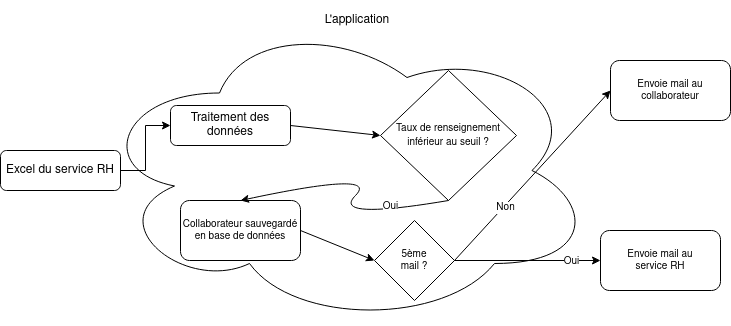
\includegraphics[width=\textwidth] {mpp-diagram.png}
  \caption {Diagram du fonctionnement de MPP Dashboard}
\end{figure}
\subsubsection{La problèmatique}
\end{sloppypar}
\end{document}

